\chapter[Cronograma]{Cronograma}

Para gerenciamento do projeto estamos utilizando a ferramenta \href{http://lappis.unb.br/redm}{Redmine}, com esta ferramenta é possível fazer o gerenciamento do projeto no contexto ágil que é o que está sendo utilizado no Projeto.

Na figura abaixo observa-se o quadro de estórias (\textit{backlog})
\begin{figure}[h]
  \centering
  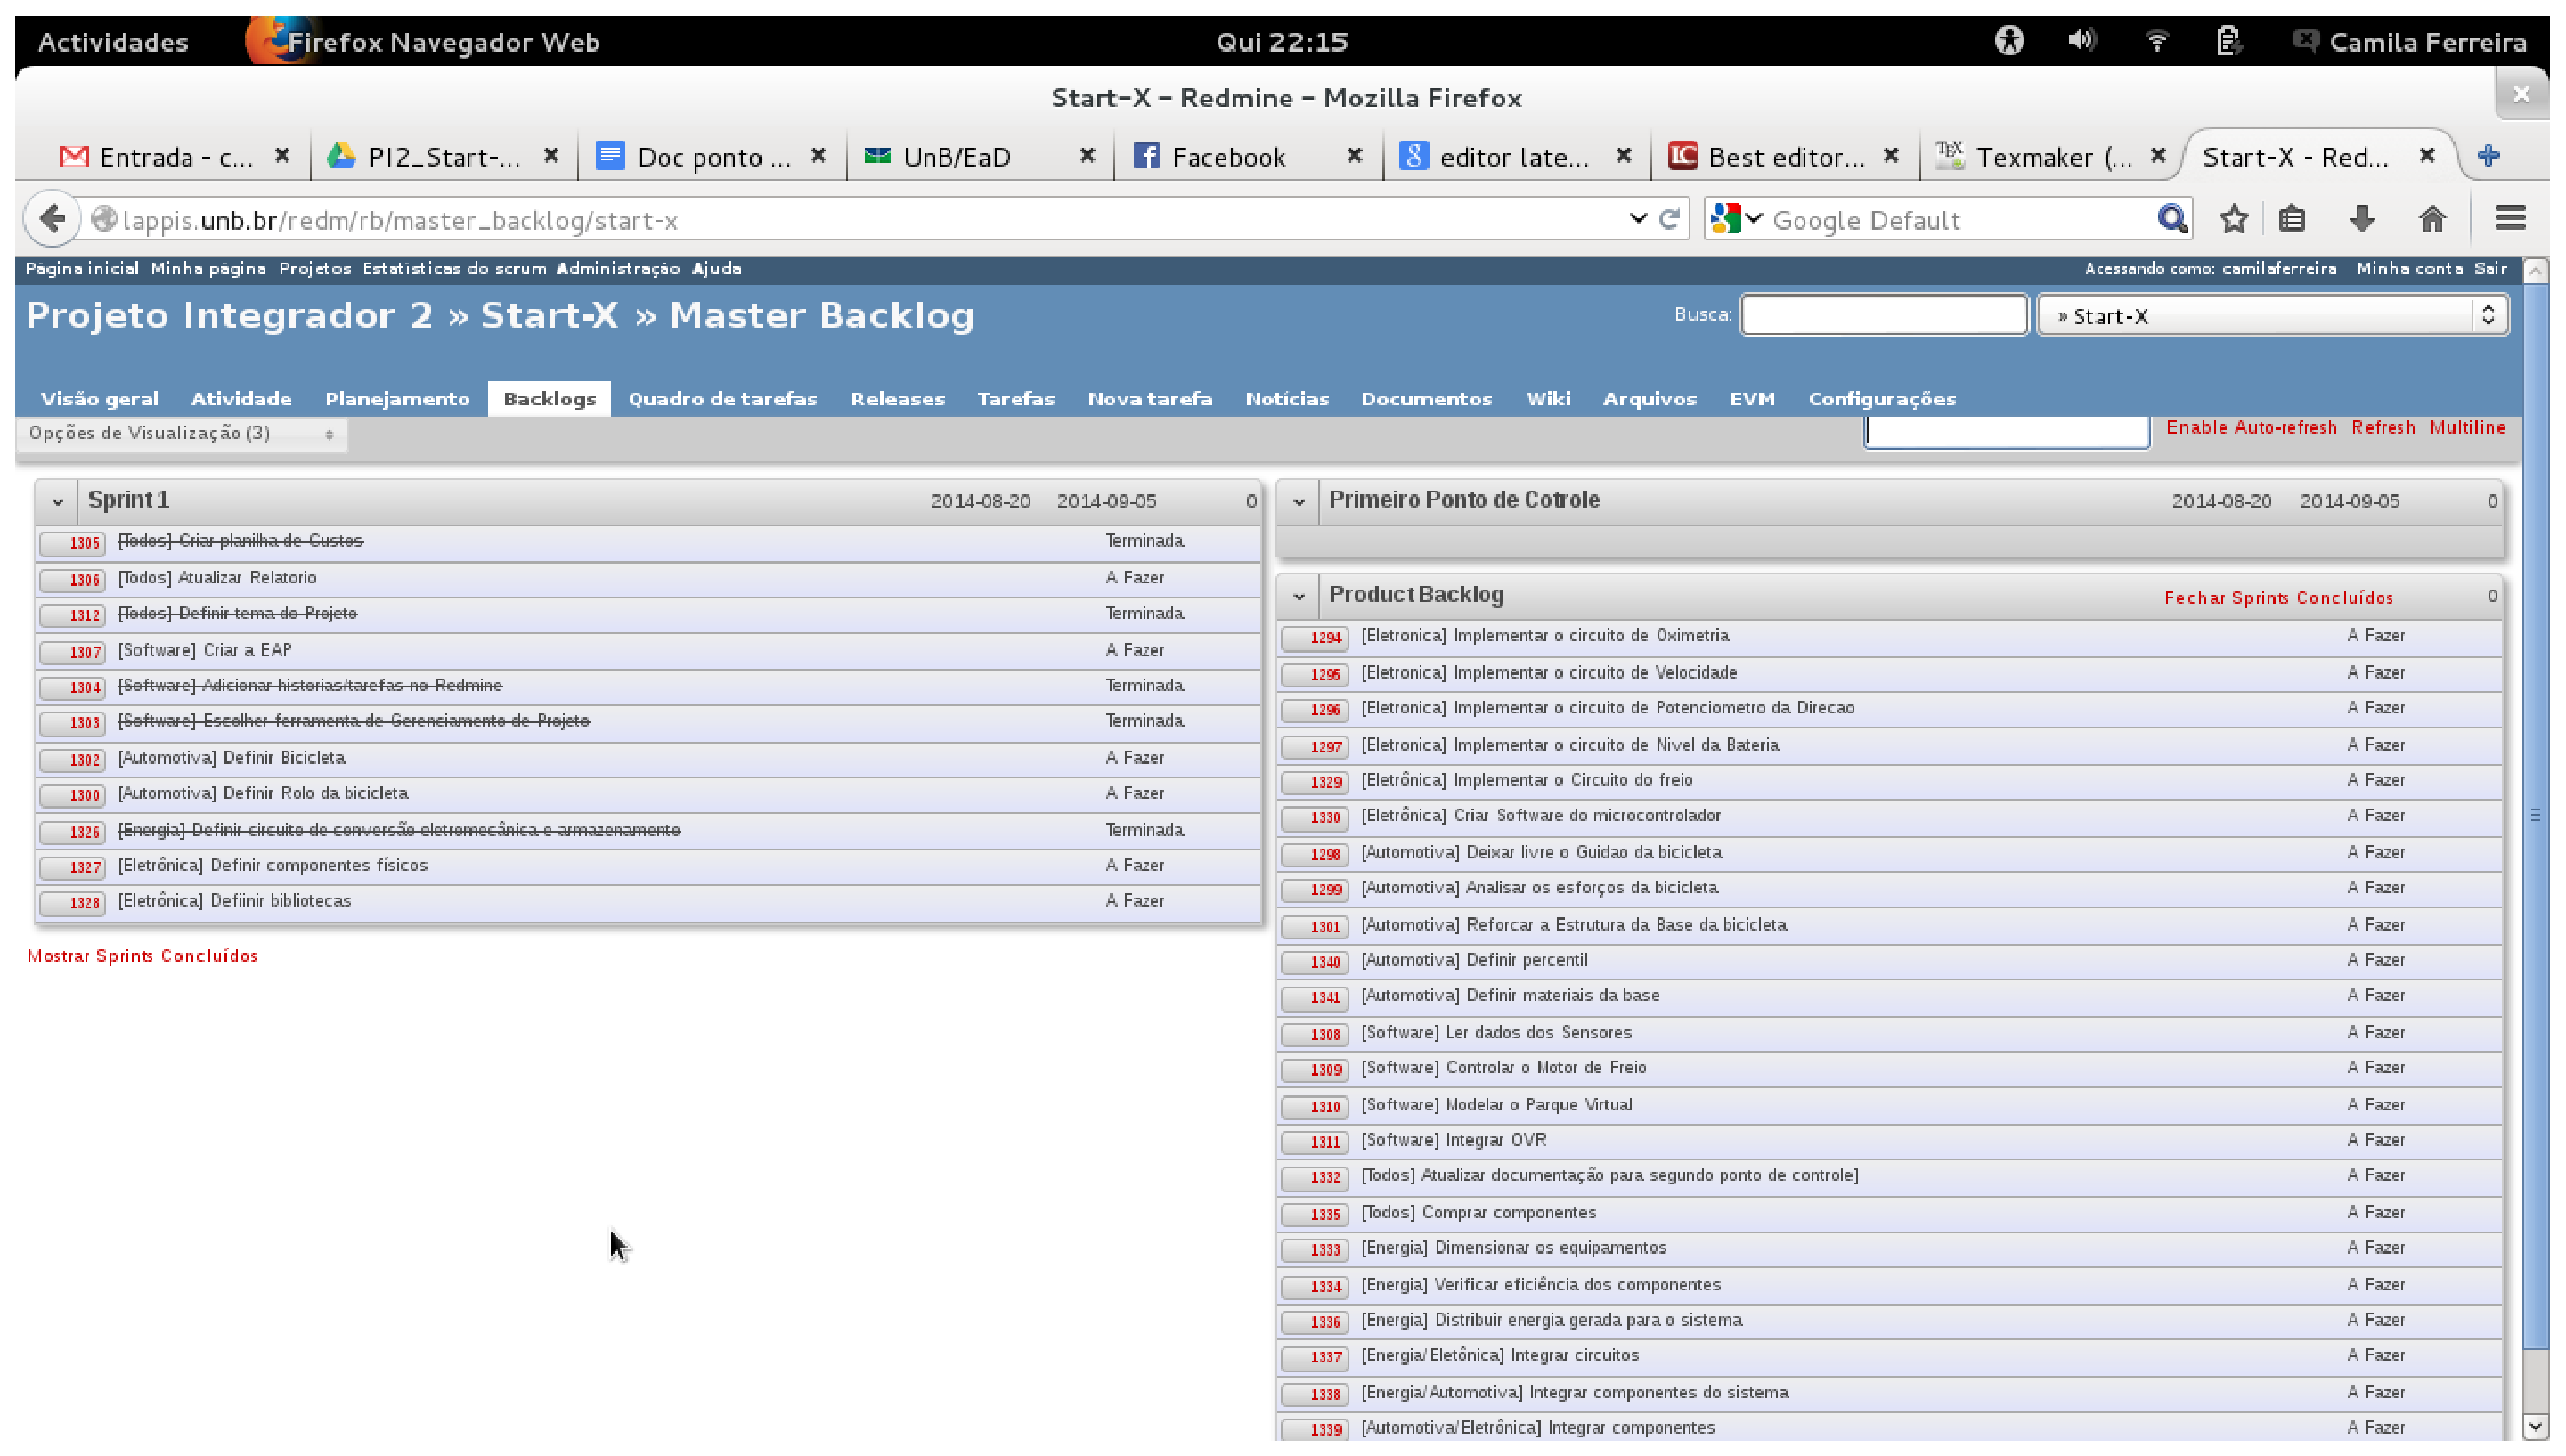
\includegraphics[width=0.8\textwidth]
      {figuras/backlogs.eps}
  \caption{Redmine e backlog do projeto}
  \label{redmine-backlog}
\end{figure}


Para gerir o projeto dividimos o projeto em 3 grandes \textit{release}s que correspondem com os 3 pontos de controle que teremos durante o semestre. A primeira \textit{release} se iniciou no primeiro dia de aula de Projeto Integrador 2 e termina no dia do primeiro ponto de controle; a segunda \textit{release} se iniciará logo após a data do segundo ponto de controle e e terminará no dia do segundo ponto de controle e a terceira \textit{release} se iniciará logo após o segundo ponto de controle terminando no dia da entrega final do produto.

\begin{figure}[h]
  \centering
  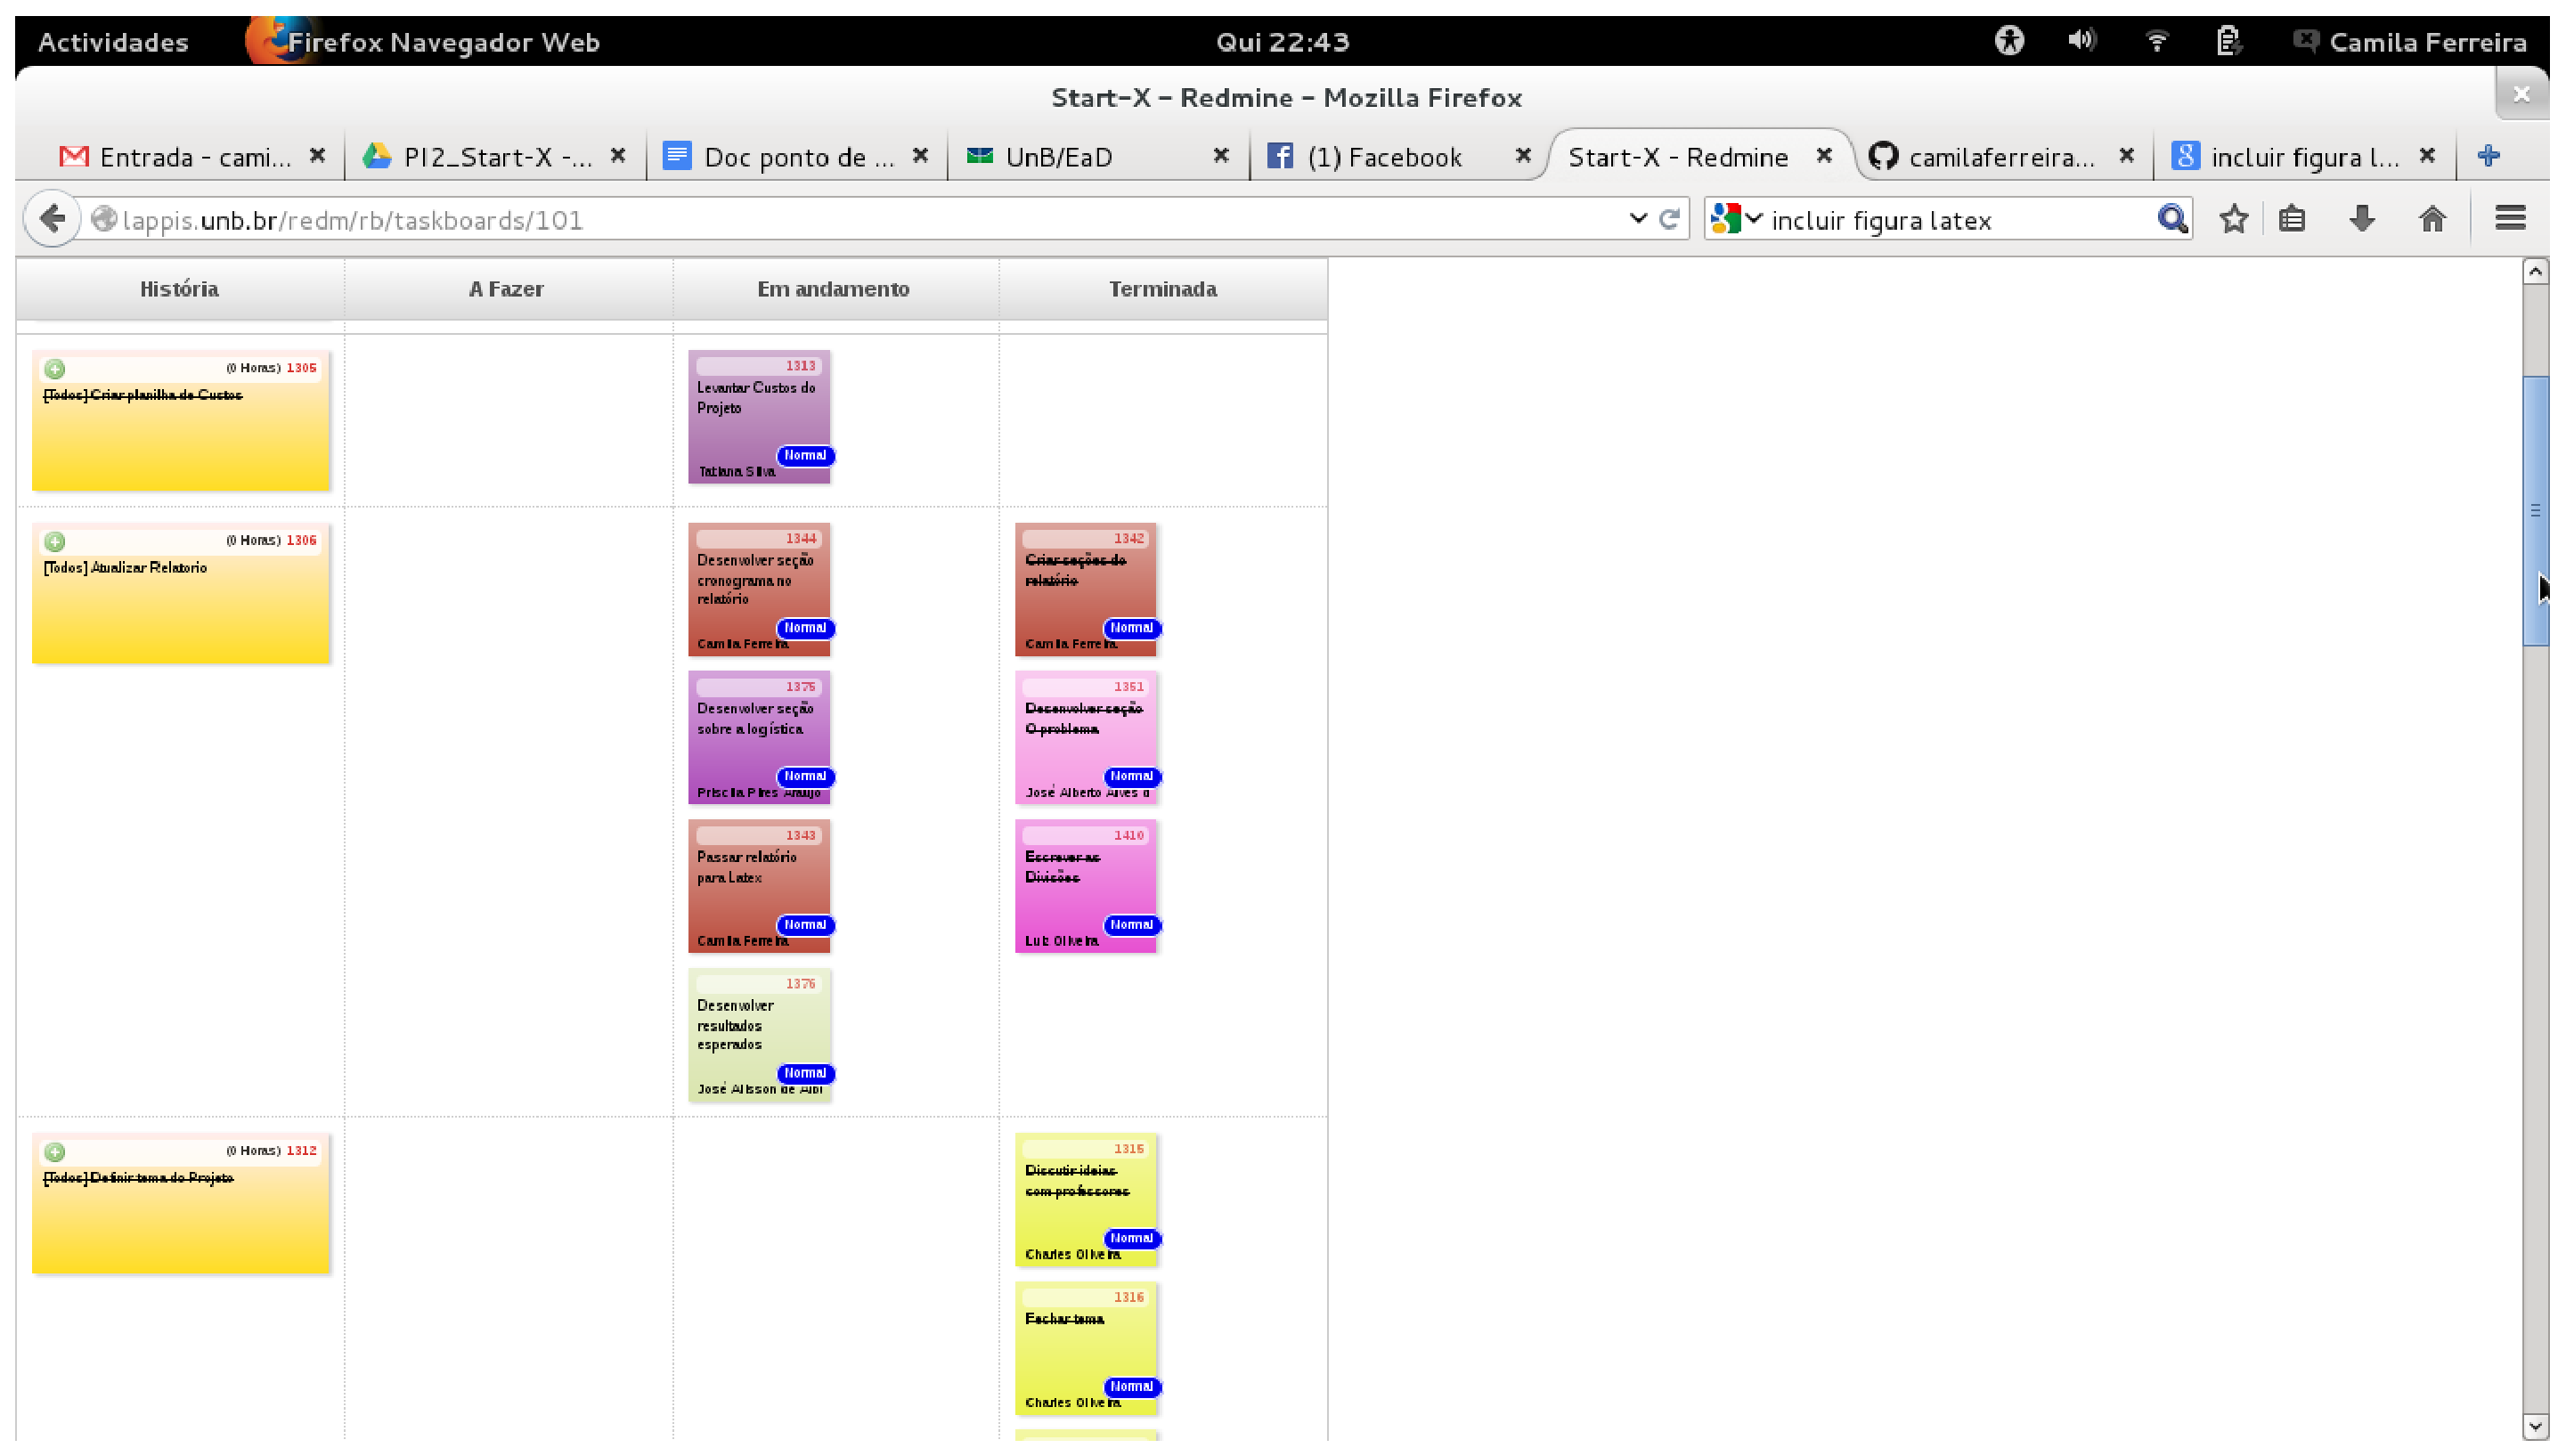
\includegraphics[width=0.8\textwidth]
      {figuras/quadrotarefas.eps}
  \caption{Quadro de tarefas}
  \label{quadro-de-tarefas}
\end{figure}
Para organizar as tarefas do projeto criamos histórias que são macrotarefas onde são posteriormente quebradas em tarefas menores. Essas tarefas são colocadas em um quadro de tarefas.


  
